% % Created 2015-09-15 Tue 11:46
% \documentclass[11pt]{article}
% \usepackage[utf8]{inputenc}
% \usepackage[T1]{fontenc}
% \usepackage{fixltx2e}
% \usepackage{graphicx}
% \usepackage{longtable}
% \usepackage{float}
% \usepackage{wrapfig}
% \usepackage{rotating}
% \usepackage[normalem]{ulem}
% \usepackage{amsmath}
% \usepackage{textcomp}
% \usepackage{marvosym}
% \usepackage{wasysym}
% \usepackage{amssymb}
% \usepackage{hyperref}
% \usepackage{color}
% \usepackage{soul}
% \tolerance=1000
% \usepackage[margin=1in]{geometry}

% \newcommand{\hilight}[1]{\colorbox{yellow}{#1}}

% %\author{Alex Ansari}
% %\date{}
% %\title{TALOS}
% %\hypersetup{
% %  pdfkeywords={},
% %  pdfsubject={},
% %  pdfcreator={Emacs 24.3.1 (Org mode 8.2.10)}}


% \begin{document}
\section{MIT Exoskeleton}
\label{mit}
\begin{refsection}[exos/mit.bib]

The MIT Exoskeleton is based on evidence from biology and passive walking devices that suggest that legged locomotion can be very efficient.  The main physical concept behind this efficiency being that there is a gait cycle for a pair of legs that naturally exchanges energy between gravity and inertia.  The main mechanical design principles center around the use of a combination of passive and active elements.  In particular, the MIT design uses {\bf springs, variable impedance joints, and powered actuators.}  The suit generally  functions as a lightweight, underactuated robot that runs in parallel to an operator and supports the weight of a payload. Additionally, the leg structure of the suit allows weight from the suit and payload to be transferred directly to the ground.

Of the several other design principles discussed, the MIT team emphasizes that joint {\bf powers scale linearly with mass}.  Also, the team points out that alterations in the operator's gait pattern have been shown to increase the physiological energy expended during locomotion.  Thus, the specifications for actuation and control for their system are extracted from the angle, torque , and power data of human walking joint patterns.     


\subsection{Actuator specifications}

The MIT exoskeleton uses a single actuator located at the hip.  The actuator is designed around a total system weight of 165 kg.  The maximum scaled hip torque for a system with this mass is approximately $-130$ Nm during the stance phase and approximately 100 Nm during the swing phase of the gait.  The hip is chosen as the actuated joint because proximal mass is metabolically less expensive in walking than distal mass.

The specific choice of actuation for the MIT exoskeleton hip joint was a {\bf linear series elastic actuator}.  This choice provided a lightweight and relatively inexpensive means of implementing force control with a bandwidth similar to that of natural muscle.  A model of the actuator is shown in Figure \ref{fig:mitSEA}.
\begin{figure}[thpb]
\centering
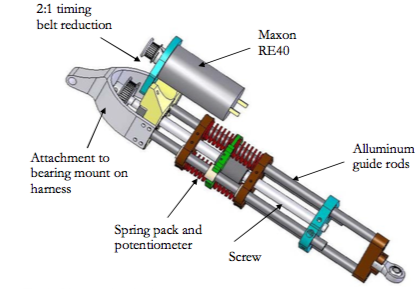
\includegraphics[width=3.in]{exos/figs/MIT/mitSEA}
  \caption{Linear series elastic actuator.}
%  \vspace{-0.2in}
 \label{fig:mitSEA}   
 \end{figure} 
Like all series elastic designs, the actuator shown in Figure \ref{fig:mitSEA} includes a spring in series with the output of the motor drive system of the actuator.  The motor-drive mechanism consists of a {\bf brushed DC motor driving a 3mm ball screw via a 2:1 reduction belt drive}.  The nut of the ball screw is coupled to the actuator output shaft via four compression die springs.  The compression of the die springs are measured using a linear potentiometer, which is how forces at the output are measured.
The team selected a {\bf 150W Maxon RE40 Brushed DC motor} for the actuator  based on the bio-mechanical data and its power and weight ratio. The force bandwidth for this actuator was characterized during both stance and swing phases of the walking gait cycle.  {\bf During stance, the bandwidth of the actuator was 35 Hz, while the bandwidth during swing was found to be 40Hz.} 
 
 \subsection{Exoskeleton Specifications}
 
 The MIT exoskeleton design has a total of fourteen degrees of freedom, three at each hip, one at each knee, two at each ankle, and one in each foot.  A cam mechanism implemented at the hip joint enables hip ab/adduction.  This system was necessary because, during abduction, there is a length difference between the operator and exoskeleton leg which results from having non-collocated centers of rotation.  The cam mechanism automatically adjusts the exoskeleton leg length such that the center of rotation of the exoskeleton hip is projected onto the biological hip center of rotation.  A picture of the MIT exoskeleton is shown in Figure \ref{fig:MITsuit}.
 \begin{figure}[thpb]
\centering
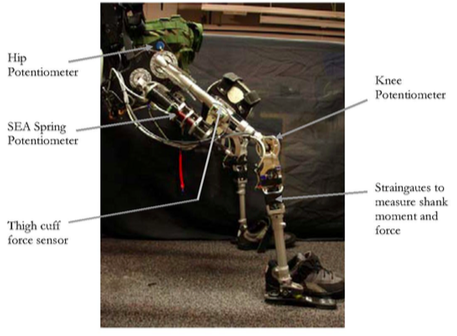
\includegraphics[width=3.in]{exos/figs/MIT/MITsuit}
  \caption{ Sensors placed on the exoskeleton leg \cite{mit_control_2006}.}
%  \vspace{-0.2in}
 \label{fig:MITsuit}   
 \end{figure} 
% 
 The interface between the suit and operator consists of shoulder straps, a compliant waist belt, thigh cuffs, and a shoe connection.  The MIT exoskeleton employs a custom-built sensor that measures the interaction force between the exoskeleton and the operator?s thigh. The sensor consisted of a spring pack, where the deflection of the passive springs was measured with a spring-loaded linear potentiometer.  

 The exoskeleton implements a {\bf variable damper knee mechanism} in the flexion/extension degree of freedom using a magnetorheological damper.  The damper can exert a {\bf maximum braking torque of 60 Nm and consums on average 1W of electrical power}.  Additionally, a linear spring at the ankles captures negative energy during dorsilflexion.  The energy stored is released during plantar flexion to add energy to the system as the foot comes off the ground. A urethane spring (247 kN/m) is used as a liner spring in a lever compression assembly.  With a lever arm of 0.0381 m, the assembly yields a spring rotary stiffness of 356 Nm/rad. 
 
 A unidirectional spring assembly is also used in the hip ab/adduction degree of freedom.  The spring allows the hip to freely abduct.  The effective rotary stiffness of the spring assembly is 96 Nm/rad in order to provide the 8 Nm required during adduction.

The suit uses a 48V battery pack and is instrumented with \textbf{rotary potentiometers} at the hip and knee.  Additionally, \textbf{strain gauges} were placed on the structure of the exoskeleton shank to measured sagittal bending moment and compression force.
 
 
 \subsection{Control Specifications}
 
The MIT exoskeleton controllers use the fact that desired actuation and active damping at the knee are functions of gait cycle.  Hence, the values of these desired functions can be determined from human walking data.  Fundamentally, the control strategy works as a state machine that uses joint angle and measured forces to implement state transitions.

\begin{figure}[thpb]
\centering
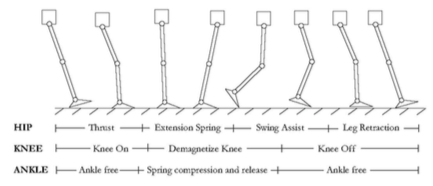
\includegraphics[width=4.in]{exos/figs/MIT/walkingCycle}
  \caption{ Summary of the actuation control of the exoskeleton leg as a function of gait cycle with an actuator at the hip and a damper at the knee. The ankle is completely passive but is included for completeness.}
%  \vspace{-0.2in}
 \label{fig:walkingCycle} 
 \end{figure} 
The walking cycle around which the MIT control scheme was designed is shown in Figure \ref{fig:walkingCycle}.  The individual control strategies in the various phases of the walking cycle are highlighted in Figure \ref{fig:walkingCycle}.  For the hip there are four distinct strategies.  During the thrust phase, the hip exerts a torque that helps to raise the center of mass of the system.  During the extension spring phase, a virtual spring stiffness allows energy to be virtually stored while the center of mass moves forward.  During the swing assist phase the virtual energy is released, resulting in a torque being applied which assists in swinging the leg forward.  Finally, in leg retraction a torque is applied to help with foot placement and weight acceptance.  A diagram that illustrates how the sensors in the shank and hip joint are used to switch between these various phases is show in Figure \ref{fig:hipControl}.
 \begin{figure}[thpb]
\centering
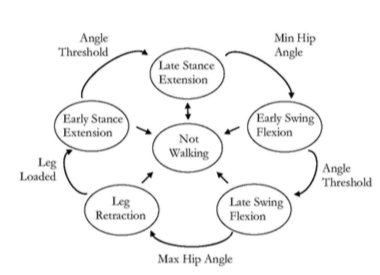
\includegraphics[width=3.in]{exos/figs/MIT/hipControl}
  \caption{State-machine diagram for the hip controller.}
%  \vspace{-0.2in}
 \label{fig:hipControl} 
 \end{figure}  
 
 The knee controller in the MIT exoskeleton effectively functions independently from he hip controller.  During knee strike, the variable damper in the knee exerts a torque proportional to the rotational velocity of the knee joint.  A residual magnetic field remains in the knee joint after it is turned off, creating a resistive torque.  The knee therefore needs to be actively demagnetized at full extension during the last phase of stance to allow it to swing freely during the subsequent swing phase.  The state machine diagram that illustrates how the various phase transitions for the knee joint were implemented using the exoskeleton's on-board sensors is in Figure \ref{fig:kneeControl}.
\begin{figure}[thpb]
\centering
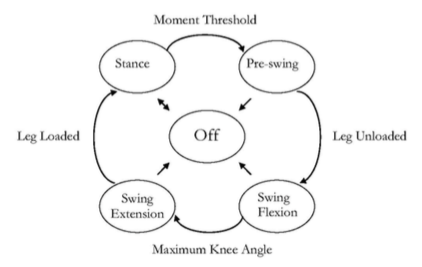
\includegraphics[width=3.in]{exos/figs/MIT/kneeControl}
  \caption{State-machine diagram for the knee controller.}
%  \vspace{-0.2in}
 \label{fig:kneeControl} 
 \end{figure}  
  
  
%  \begin{figure}[thpb]
%\centering
%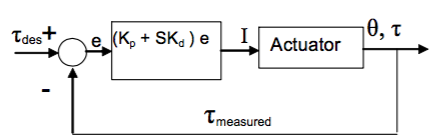
\includegraphics[width=3.in]{figs/torqueCon}
%  \caption{}
%  \vspace{-0.2in}
% \label{fig:IHMCTOR}   
% \end{figure}
% 
 
 
 \subsection{Assessment and Recommendations}
 
 The MIT hardware and control system present a very well designed and thought-out system that focuses primarily on efficiency in design.  The series elastic linear ball screw hardware design seems to be a very smart way to implement efficient drives as well as to perform high fidelity force control.  The use of a strain gauge in the shank was also a novel means of measuring ground reaction forces.  This design may offer benefits in terms of repeatability over different operators as foot fall patterns for different users may include significant variations.
 
 The details on the controllers were somewhat sparse in the sense that, at least in \cite{mit_control_2006}, the exact means through which the added torques were derived was not provided.  Overall though, the controllers were intelligently designed in the sense that they explicitly took the biomechanics of walking into account in their design and implementation.  A similar approach for a variety of different behaviors may be very beneficial to the TALOS project.  
 
 The hardware specifications and associated figures in this section were taken from \cite{mit_design_2006}.  The discussion on control design and and the associated figures therein are respectively based on and taken from \cite{mit_control_2006}. 
 
 
 \printbibliography[heading=subbibliography]

\end{refsection}

 
% \end{document}

% Conor James Walsh and Daniel Paluska and Kenneth Pasch and William Grand and Andrew Valiente and Hugh Herr, "Development of a lightweight, underactuated exoskeleton for load-carrying augmentation," Proceedings of the 2006 IEEE International Conference on Robotics and Automation, 2006, pp. 3485 - 3491.

% Conor James Walsh and Kenneth Pasch and Hugh Herr, "An autonomous, underactuated exoskeleton for load- carrying augmentation, " International Conference on Intelligent Robots and Systems, 2006, pp. 1410-1415.

%%% Local Variables:
%%% mode: latex
%%% TeX-master: "../survey"
%%% End:
